\documentclass{article}

% LP4FM double-blind workshop submission using the NeurIPS 2026 style.
\usepackage[dblblindworkshop]{neurips_2026}
\workshoptitle{Linguistic Principles for Foundation Models}

\usepackage[utf8]{inputenc}
\usepackage[T1]{fontenc}
\usepackage{hyperref}
\usepackage{url}
\usepackage{booktabs}
\usepackage{amsmath,amssymb,amsthm}
\usepackage{microtype}
\usepackage{xcolor}
\usepackage{graphicx}
\usepackage{multirow}
\usepackage{tabularx}
\usepackage{float}
\hypersetup{hidelinks}

\newtheorem{proposition}{Proposition}
\newtheorem{definition}{Definition}
\newtheorem{remark}{Remark}

\title{Descriptions as Controllers: Identifiability and Saturation of Belief-Source Access in Language Models}

\author{Anonymous Authors}

\begin{document}

\maketitle

\begin{abstract}
Two descriptions can encode the same false-belief world yet make a language
model answer from different sources. Accuracy alone cannot reveal whether the
answer follows the queried agent, reality, another agent, or a distractor. We
make this hidden controller identifiable by crossing fixed worlds with typed
competitors and linguistic changes to discourse order, reference, voice,
embedding locality, and source attribution. What first appears to be erratic
prompt sensitivity becomes a structured source-routing effect. A reportative
reversal then suggests a stronger hypothesis: linguistic constraints share an
accessibility bottleneck rather than imposing independent costs. Freezing the
primitive costs yields a risky prediction for unseen compound constructions.
Independent latent worlds confirm strict subadditive composition in
Qwen2.5-7B-Instruct for both reportative and factive constructions. Frozen
transfer to Qwen3-8B and matched Qwen2.5-7B Base preserves partial
control-relative shape but not the directional residual. An affine-gain
invariance result rules out the explanation that these checkpoints merely
express the same law at a smaller logit scale. The resulting contribution is a
checkpoint-sensitive behavioral theory of how descriptions route answers among
typed sources, not a claim about a unique neural circuit or a causal effect of
instruction tuning.
\end{abstract}

\section{Introduction}

Consider two descriptions of the same world. The agents, object movements,
and false belief are identical; only the linguistic route changes. The relevant
state may appear earlier or later, under a name or an ambiguous pronoun, in an
active clause or inside an impersonal report. A language model can reverse its
answer even though the world has not changed. The usual diagnosis is prompt
brittleness. Our starting point is different: perhaps the description changed
\emph{which source was allowed to control the answer}.

Standard Theory-of-Mind evaluation cannot separate these possibilities. A
correct false-belief answer is compatible with following the queried agent,
copying reality, tracking another agent, or exploiting a cue that happens to
agree with the target. Semantics-preserving perturbations expose this fragility
\citep{ullman2023trivial,shapira2024cleverhans}, but a catalog of reversals still
identifies only the winning answer. It does not identify the controller that
made that answer win.

We treat a description as a \emph{binding controller}: a linguistic interface
that regulates access to source-indexed states while the model arbitrates among
the queried agent's belief, reality, another agent's state, and an object
distractor. This reframes the problem from ``does the model contain belief
information?'' to ``when does a description make one source govern the
answer?'' The framing connects model evaluation to discourse accessibility,
where order and referring form alter which entities or propositions remain
available for interpretation
\citep{gundel1993givenness,grosz1995centering,webster-nothman-2016-using}.

This change of object turns two failures into the main scientific clues. First,
pooled wording effects reverse across item pools. They become systematic only
after we expose the \emph{typed conflict topology}: whether the target source
competes with reality, another agent, or both. Second, one otherwise successful
linguistic contrast reverses when each event is placed under a reportative
predicate. The facts remain present, but their attributed route to the answer
changes. Together these observations suggest that linguistic form controls
source access rather than contributing a context-free answer bias.

That hypothesis makes a quantitative prediction. Passive voice, event-local
embedding, and source attribution each reduce the target source's influence.
If the reductions are independent, their costs should add in an unseen compound
construction. If they act through a shared accessibility bottleneck, the second
constraint should have less room to operate once the first route is limiting.
The latter predicts a positive compound-minus-additive residual. We freeze the
primitive costs before observing the compounds and confirm the prediction on
new latent worlds in Qwen2.5-7B-Instruct.

The law is not universal across the checkpoints we test, and that failure
sharpens rather than dissolves the result. The identical frozen protocol on
Qwen3-8B and matched Qwen2.5-7B Base retains partial control-relative predictor
advantages but not the directional residual. A positive affine change of
readout scale would preserve residual sign and normalized geometry; it does
not. The checkpoints therefore differ in the \emph{shape} of linguistic-source
composition, not merely in confidence or logit amplitude.

The paper's argument has three parts. We first introduce a typed source-control
object that makes controller identity behaviorally observable under fixed
semantics. We then derive and independently test a source-accessibility
saturation law for compound linguistic constraints. Finally, we use frozen
cross-checkpoint failures and an affine-gain invariance result to delimit the
law as checkpoint-sensitive. This supports a falsifiable behavioral theory of
language-mediated source routing. It does not identify a unique aggregation
operator, a hidden-state circuit, a causal effect of instruction tuning, or a
human psycholinguistic universal.

\section{Related Work}

\paragraph{Theory-of-Mind evaluation in language models.}
Question-answering benchmarks operationalize belief attribution through
controlled stories \citep{le-etal-2019-revisiting}, while conversational
benchmarks test information asymmetry and consistency across related questions
\citep{kim-etal-2023-fantom}. Subsequent stress tests show that high average
accuracy can coexist with failures under trivial or adversarial alterations
\citep{ullman2023trivial,shapira2024cleverhans}. These studies motivate robust
evaluation, but typically retain answer correctness as the principal object.
Our work instead holds story semantics fixed, types the competing answer
sources, and estimates which linguistic description controls arbitration among
them. It therefore addresses controller identification rather than proposing a
broader ToM benchmark.

\paragraph{Discourse accessibility and reference.}
The Givenness Hierarchy links referring form to assumptions about cognitive
status \citep{gundel1993givenness}, and Centering Theory models local discourse
coherence through ranked discourse entities \citep{grosz1995centering}.
Computational coreference work similarly uses mention accessibility to improve
antecedent selection \citep{webster-nothman-2016-using}. Our intervention axes---
description order, explicit names versus ambiguous pronouns, and role labels---
draw on this tradition, but our dependent variable is not human interpretation
or coreference accuracy. We ask how these forms alter a foundation model's
typed answer margin under controlled conflict.

\paragraph{Embedding predicates, factuality, and source commitment.}
Clause-embedding predicates support systematic inferences about the factual
status and source of embedded events. Large-scale lexicosyntactic studies show
that neural models acquire some of these patterns while remaining sensitive to
the lexical and syntactic realization \citep{white-etal-2018-lexicosyntactic}.
Pragmatic evaluations further find that contextual event factuality is not
captured by lexical entailment alone \citep{jiang-de-marneffe-2021-thinks}. We
use reportative and factive predicates as controlled accessibility constraints:
the relevant question is not whether the embedded proposition is globally
entailed, but whether its source remains effective in typed answer arbitration.

\paragraph{Behavioral and compositional evaluation.}
Minimal-pair suites \citep{warstadt-etal-2020-blimp-benchmark}, behavioral test
matrices \citep{ribeiro-etal-2020-beyond}, and contrast sets
\citep{gardner-etal-2020-evaluating} all argue that aggregate test accuracy is
insufficient for characterizing model behavior. Compositional benchmarks test
whether primitive linguistic operations generalize to unseen combinations
\citep{kim-linzen-2020-cogs}. We combine these principles but make the
composition hypothesis quantitative: primitive construction costs are frozen
before unseen compounds are evaluated, and the additive null is rejected by a
preregistered compound-minus-additive inequality. This identifies a behavioral
subadditivity class rather than merely cataloguing another sensitivity.

\paragraph{Language representation as a control interface.}
Recent work argues that language representation design can alter the activation
and organization of model knowledge even without parameter updates
\citep{yang2026schema}. Our results provide a narrow empirical law for that
broader proposal. In controlled belief-binding worlds, representation design
changes source access, but simultaneous linguistic constraints exhibit
saturation rather than independent gains or losses.

\section{Methodology}

% Plan: State the identification principle that organizes all experiments.
Our design follows one identification principle: change the linguistic route to
a belief while holding the world fixed, then change the identity of the
belief's competitors while holding the linguistic contrast fixed. The first
intervention establishes that form matters; the second reveals what that form
controls. We separate hypothesis formation from held-out prediction and
independent confirmation so that a descriptive sensitivity cannot promote
itself into a compositional law. The complete experimental inventory appears in
Appendix~\ref{app:evidence-inventory}.

\subsection{The answer is a typed competition}

% Plan: Define the latent world and explain why typed candidates identify source competition.
Each latent world specifies a queried agent, a comparison agent, an object, an
initial location, a true final location, and agent-indexed information states.
The event sequence is generated once and reused across all surface forms. Its
answer candidates are typed as the queried agent's belief, reality, the
comparison agent's state, or an object distractor. We construct role conflict,
object conflict, and joint role-plus-object conflict by changing which typed
competitors disagree with the instructed source. Candidate strings remain
invariant within a latent-world block. Consequently, a changing margin cannot
be attributed to a changing ground truth or answer vocabulary; it records
which source defeats which competitor.

% Plan: Make explicit the invariant checks that prevent surface changes from changing the task.
Every crossed block is audited for an identical event manifest, queried target,
candidate set, and instruction target. All 30 worlds in the same-item,
multi-realization, factorial, and first compound analyses pass these invariance
checks. The final confirmation uses 20 newly generated worlds with zero
normalized latent-signature overlap with the earlier pool. The rejected
cross-pool main-effect test likewise uses zero item overlap. A replay-equivalent
intermediate pool with complete identity overlap is retained only as an
execution check and is excluded from scientific replication claims.

\subsection{Descriptions change the route, not the world}

% Plan: Introduce the high-level linguistic interventions and their theoretical roles.
The first intervention family varies description order, reference form,
negation/evidential wording, and role labels. These contrasts manipulate which
source is introduced first, how explicitly its discourse referent is resolved,
and whether competing sources are excluded or the target evidence is
affirmatively licensed. The full inventory contains 10 controlled arms plus the
original description (Appendix~\ref{app:linguistic-arms}). Description order,
reference form, and negation/evidential wording are preregistered confirmatory
axes in the topology cross; role label versus name is retained as exploratory.

% Plan: Explain the realization and construction manipulations that separate robustness from accessibility.
We next re-express the same event structure as a canonical narrative,
structured event log, event-wise report, or compact indirect report. The
critical construction family crosses active versus genuine passive voice,
global versus event-local embedding, and reportative versus factive predicates.
These operations alter discourse prominence, grammatical argument realization,
embedding locality, or source commitment without changing the event sequence.
The compound test holds out all passive-by-embedding combinations while
estimating primitive voice and locality effects from the non-compound cells.

% Plan: Document exact-length and candidate-token controls.
We evaluate target context lengths of 1,024 and 2,048 tokens. Neutral padding is
inserted outside the answer-bearing event block, and exact length is checked
with the model tokenizer after the complete description and target block are
assembled. Every source decision reports full exact-length coverage. All
confirmatory answer candidates are required to be single tokens, preventing
multi-token normalization or stopping decisions from entering the margin.

\subsection{A margin identifies the winning source}

% Plan: Specify the model and inference procedure without implying training or hidden-state access.
Experiments use a fixed Qwen2.5-7B-Instruct checkpoint
\citep{qwen2024qwen25}. No weights are updated and no free-text decoding is
used for the primary evidence. The scorer obtains next-token logits at the
answer position and evaluates every typed candidate under the same prompt. The
checkpoint, tokenizer, data type, device map, and source manifests are fixed
before each confirmatory matrix; implementation details appear in
Appendix~\ref{app:reproducibility}.

% Plan: Define the answer-interface binding margin.
For prompt $x_i(c,T,a)$, let $\ell_i(y)$ be the next-token log probability of
candidate $y$. If $y_i^\star$ is the source licensed by the instruction and
$\mathcal{Y}_i^{-}$ is the set of typed competitors, the binding margin is
\begin{equation}
M_i(a,T,c)=\ell_i(y_i^\star)-\max_{y\in\mathcal{Y}_i^{-}}\ell_i(y).
\label{eq:binding-margin}
\end{equation}
A positive margin means that the instructed source wins the answer interface;
the magnitude records its distance from the strongest typed competitor. This
definition is intentionally behavioral: it does not assume a localized belief
representation or source-monitoring circuit.

% Plan: Define the paired linguistic effect and topology interaction.
For a linguistic contrast with arms $a^+$ and $a^-$, define
\begin{equation}
\Delta_i(T,c)=M_i(a^-,T,c)-M_i(a^+,T,c).
\label{eq:language-effect}
\end{equation}
Our primary topology estimand is the excess effect under joint conflict,
\begin{equation}
\Gamma_i(c)=\Delta_i(T_{\mathrm{role+object}},c)
-\tfrac{1}{2}\left[\Delta_i(T_{\mathrm{role}},c)
+\Delta_i(T_{\mathrm{object}},c)\right].
\label{eq:topology-interaction}
\end{equation}
This difference-in-differences removes the average single-conflict effect and
isolates how language form responds to concurrent typed competitors.

\subsection{Falsification before confirmation}

% Plan: Explain how each experiment changes the epistemic status of the claim.
Each transition in the argument is triggered by a failed explanation. Pooled
language effects are tested on an item-disjoint pressure pool before typed
conflict is introduced. The typed interaction is then challenged across four
surface realizations; its reportative reversal motivates the accessibility
hypothesis. Primitive voice and locality costs are estimated in a factorial and
frozen before unseen compounds are scored. Only after those compounds suggest a
saturating class do we register its residual sign and predictive controls and
test them on 20 new latent worlds. Later evidence therefore answers a new
question rather than adding rows to an earlier grid.

% Plan: State the negative controls and no-promotion rules.
Three controls prevent a descriptive pattern from being mistaken for
independent evidence.
First, the replay-equivalent pool is not counted as independent evidence.
Second, role label versus name is not promoted with the preregistered axes.
Third, a held-out additive predictor must beat the no-voice control before
additive composition can be claimed. It does not; the residual pattern is used
only to formulate the subsequent saturation hypothesis. Independent
confirmation then tests that hypothesis without selecting among saturation
operators.

\subsection{Uncertainty and confirmatory criteria}

% Plan: Define the cluster bootstrap and why the latent world is the sampling unit.
All estimands are first reduced within latent world by averaging the two context
lengths. We use nonparametric item-cluster bootstrap intervals, resampling
latent worlds while preserving every topology, construction, length, and
instruction arm belonging to a world. Unless stated otherwise, intervals are
95\% percentile intervals from 8,000 resamples with fixed analysis seeds. This
avoids treating correlated surface realizations as independent observations.

% Plan: State each confirmatory gate explicitly.
The topology claim requires the preregistered direction and a directional
confidence interval for all three primary axes, with the same direction at both
context lengths. Cross-realization confirmation requires an aggregate
directional interval and the predicted sign in at least three of four
realization families. Independent saturation requires a positive lower interval
bound in both reportative and factive families, together with improvements of
both weakest-link and average-saturation predictors over the frozen additive
null. Full cell-level results and decision criteria are reported in the
appendix.

\section{Experiments and Results}

\subsection{Experimental design and statistical unit}

The experiments are organized as a sequence of identification and prediction
tests rather than as an undifferentiated prompt grid. We begin with 80 latent
worlds for surface-axis discovery and a separate 80-world pressure pool for
falsification. A 30-world same-item topology matrix then crosses role, object,
and joint conflict. The same 30 worlds are rendered in four realization
families and in a construction factorial that estimates primitive voice,
locality, and source-attribution costs. We hold out 30 passive-by-embedding
forms for compound prediction and reserve 20 new latent worlds for independent
saturation confirmation. Across all matrices this produces 16,700 scored rows,
but the latent world, not the row, is the sampling unit.

The primary linguistic axes are description order, reference form, and
negation/evidential wording. Role label versus name is retained as a control and
exploratory contrast rather than promoted after inspection. Every world is
evaluated at 1,024 and 2,048 tokens with the same typed candidate interface;
neutral padding is placed outside the answer-bearing event block. This design
separates semantic invariance from surface realization and prevents context
length or candidate normalization from becoming an unreported source of
variation.

For each latent world, we average the two context lengths before resampling and
use an item-cluster bootstrap that preserves all topology, construction, and
instruction-arm rows belonging to that world. The pressure-pool reversal,
typed-topology interaction, held-out residual, and cross-checkpoint residual
therefore answer different questions. A result is promoted only when its
predeclared directional or control gate is satisfied; a failed gate remains a
boundary result rather than a reason to refit the contrast.

\subsection{Average wording effects conceal the controller}

The most economical account of prompt sensitivity is that each linguistic form
contributes a stable amount of evidence for the intended belief. Our first test
rejects that account. Description order and reference form change direction or
collapse when evaluated on an item-disjoint pressure pool. A wording form
therefore does not carry a portable, context-free weight; the complete estimates
and uncertainty intervals are reported in Appendix~\ref{tab:cross-pool}.

The first gate is a direct portability test. If a wording form carried a stable
language-level weight, its paired effect should preserve direction on the
item-disjoint pressure pool. It does not: description order reverses and
reference form collapses, while the designated controls also fail their frozen
criteria (Table~\ref{tab:main-cross-pool}). This negative result is informative
because it rules out the simplest explanation before any typed conflict probe is
introduced.

\begin{table}[H]
\centering
\footnotesize
\setlength{\tabcolsep}{3pt}
\begin{tabularx}{\columnwidth}{Xlrrrc}
\toprule
Axis & Arm & Discovery & Pressure & Sign stable & Gate \\
\midrule
Description order & Primary & -2.132 & 4.678 & No & Fail \\
Reference form & Primary & 0.705 & -0.227 & No & Fail \\
Negation/evidence & Control & 0.541 & 4.143 & Yes & Control fail \\
Role label/name & Control & -0.328 & -1.238 & Yes & Control fail \\
\bottomrule
\end{tabularx}
\caption{Cross-pool falsification of a portable wording effect. The discovery
and item-disjoint pressure pools use the same linguistic contrasts but different
latent worlds. The two preregistered primary axes reverse or collapse, so no
context-free language weight is promoted. The complete intervals and gate
definitions are reported in Appendix~D.}
\label{tab:main-cross-pool}
\end{table}


The failure points to a hidden variable: the identity of the source competing
with the target. We expose it by crossing new latent worlds with role, object,
and joint role-plus-object conflict while preserving the event sequence,
candidate vocabulary, and linguistic contrast. The joint-minus-average-single
interaction is directional for all three preregistered linguistic axes and
remains so at both context lengths (Appendix~\ref{tab:same-item}).

Table~\ref{tab:key-estimates} places the evidence on a common scale. The
typed-conflict interactions are estimated on the original worlds, whereas the
cross-realization and saturation entries are evaluated on distinct realization
families or new latent worlds. This is an evidence ladder, not a ranking of
prompt effects: each row changes the epistemic status of the claim.

\begin{table}[H]
\centering
\small
\begin{tabularx}{\columnwidth}{Xrrl}
\toprule
Estimand & Mean & Bootstrap interval & Evidence unit \\
\midrule
Order $\times$ topology & 6.722 & [5.697, 7.747] & same-world \\
Reference $\times$ topology & -1.062 & [-1.724, -0.409] & same-world \\
Negation/evidence $\times$ topology & 3.706 & [2.875, 4.527] & same-world \\
Order across realizations & 4.551 & [3.907, 5.152] & 4 realizations \\
Reference across realizations & -1.006 & [-1.474, -0.530] & 4 realizations \\
Reportative saturation & 4.609 & [2.646, 6.447] & new worlds \\
Factive saturation & 3.771 & [2.274, 5.228] & new worlds \\
\bottomrule
\end{tabularx}
\caption{Key estimates in the argument. Topology effects are joint-minus-average-single interactions; saturation effects are compound-minus-additive residuals. Intervals are 95\% percentile item-cluster bootstrap intervals.}
\label{tab:key-estimates}
\end{table}


This interaction changes the interpretation of the original instability. The
same description can help when the target competes with one source and hurt when
it competes with two. Linguistic form is not simply shifting an answer score; it
is changing arbitration among typed sources. The object to explain is therefore
\emph{source routing under conflict}, not average prompt robustness.

\subsection{A reportative reversal reveals an accessibility bottleneck}

If typed source routing is real, it should survive changes in surface
realization while remaining sensitive to constructions that alter source
access. We render the same worlds as canonical narratives, structured event
logs, event-wise reports, and compact indirect reports. Aggregate topology
effects remain directional for the main language axes, and order and reference
preserve their signs across the realization families
(Appendix~\ref{tab:multitemplate}).

The informative case is the exception. Under event-wise reportative embedding,
the negation/evidential interaction reverses direction. The event facts and
answer candidates are unchanged, but each fact now reaches the query through an
attributed report. The reversal is hard to explain as generic template
sensitivity: it specifically implicates the route from a described source to
the answer interface.

We test that interpretation by separating three ways of restricting the route:
grammatical demotion through passive voice, event-local embedding, and
reportative rather than factive attribution. Relative to the active unembedded
form, passive voice and event-local embedding each reduce the topology-moderated
effect; locality is additionally more damaging under reportative than factive
attribution. These contrasts isolate distinct linguistic restrictions on source
access without asserting that the model contains an explicit scalar
accessibility variable (Appendix~\ref{tab:factorial}).

\begin{figure*}[t]
    \centering
    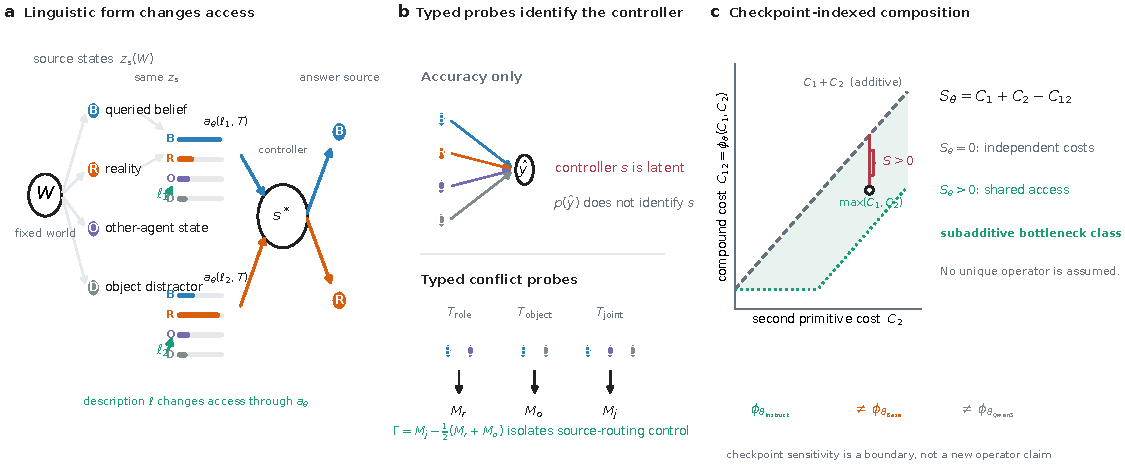
\includegraphics[width=\textwidth]{figures/figure_source_accessibility_bottleneck.pdf}
    \caption{\textbf{A theory of linguistic source control.} (a) A fixed
    latent world supplies typed source states; linguistic form changes their
    access vector and therefore the source selected at the answer interface.
    (b) Accuracy alone leaves the controller unidentifiable, whereas typed
    conflict probes produce the source-routing interaction $\Gamma$. (c) The
    compound cost lies in a subadditive class between $\max(C_1,C_2)$ and
    $C_1+C_2$. The checkpoint comparison in the final paragraph tests whether
    this composition class transfers; its complete quantitative evidence is
    reported in Table~\ref{tab:main-checkpoint-boundary}.}
    \label{fig:main}
\end{figure*}

\subsection{The bottleneck predicts subadditive composition}

The accessibility account becomes scientifically useful only if it predicts an
unseen construction. Let $c_0$ be the active, unembedded baseline, and define a
construction's behavioral accessibility cost as its loss in topology-moderated
source control relative to $c_0$. Independent restrictions predict that the
cost of passive voice and local embedding should add. A shared bottleneck
predicts overlap: once one route is limiting, the other cannot impose its full
standalone cost.

\input{../../results/oral_readiness_pack_20260707/source_accessibility_saturation_theory/source_accessibility_saturation_theorem}

Proposition~\ref{prop:cost-residual} turns this contrast into an observable
inequality. Additivity predicts $S=0$; shared saturation predicts $S>0$. The
claim is deliberately about a subadditive composition class, not a unique
weakest-link, soft-min, or neural aggregation operator.

We freeze primitive voice and locality costs before evaluating unseen
passive-by-embedding compounds. The additive model overshoots the compound
response systematically, while the saturating predictors reduce this error.
The weakest-link predictor does not reliably separate from average saturation.
The held-out compounds therefore reject independent costs and motivate a
saturating class, while leaving the operator unidentified
(Table~\ref{tab:main-heldout} and Appendix~\ref{tab:model-comparison}).

\begin{table}[H]
\centering
\footnotesize
\setlength{\tabcolsep}{3pt}
\begin{tabularx}{\columnwidth}{Xrrrrrr}
\toprule
Unseen compound & Actual & Additive & Residual & Interval & Additive MAE & No-voice MAE \\
\midrule
Passive + global reportative & -0.142 & -0.364 & 0.222 & [-0.615, 1.026] & 1.835 & 2.930 \\
Passive + local reportative & -0.757 & -3.426 & 2.668 & [2.026, 3.354] & 2.753 & 1.518 \\
Passive + global factive & 0.120 & -1.034 & 1.154 & [0.350, 1.979] & 1.967 & 2.381 \\
Passive + local factive & -0.654 & -3.066 & 2.411 & [1.707, 3.134] & 2.486 & 1.786 \\
\bottomrule
\end{tabularx}
\caption{Held-out compound test. Primitive voice and locality costs are frozen before scoring these four passive-by-embedding compounds. Three residual intervals exclude zero in the positive direction, rejecting independent additive costs. Intervals are 95\% percentile item-cluster bootstrap intervals.}
\label{tab:main-heldout}
\end{table}


\subsection{New worlds confirm the law; new checkpoints delimit it}

The decisive test freezes the residual direction and both saturating controls,
then evaluates them on latent worlds with no signature overlap with the earlier
pool. No primitive cost or operator is selected on these worlds. The compound
response lies above the additive prediction for both reportative and factive
constructions, and both saturating predictors improve over additivity. The new
worlds therefore confirm a checkpoint-internal law: concurrent linguistic
restrictions impose strictly subadditive behavioral costs in
Qwen2.5-7B-Instruct. The complete quantitative audit is provided in
Appendix~\ref{tab:independent-saturation}.

We next freeze the complete protocol and change only the checkpoint. Qwen3-8B
and matched Qwen2.5-7B Base do not reproduce the directional residual; their
intervals include zero. Yet both checkpoints retain a control-relative
preference for saturating predictors over additivity. What transfers is
therefore not the strong law itself, but a weaker structural preference
 (Table~\ref{tab:main-checkpoint-boundary}).

\begin{table}[H]
\centering
\small
\begin{tabular}{lrrcc}
\toprule
Checkpoint & Residual & Interval & Predicate gates & Control gates \\
\midrule
Qwen2.5-7B-Instruct & 4.190 & [2.931, 5.401] & 2/2 & 2/2 \\
Qwen3-8B & 0.250 & [-0.095, 0.580] & 0/2 & 2/2 \\
Qwen2.5-7B Base & -0.184 & [-0.453, 0.107] & 0/2 & 2/2 \\
\bottomrule
\end{tabular}
\caption{Frozen checkpoint boundary. The directional saturation residual is specific to Qwen2.5-7B-Instruct, whereas both alternate checkpoints retain the weaker control-relative predictor preference. Intervals are 95\% percentile item-cluster bootstrap intervals.}
\label{tab:main-checkpoint-boundary}
\end{table}


Could this be the same composition law expressed at lower confidence?
Proposition~\ref{prop:affine-gain-invariance} shows that a positive affine
readout map must preserve residual sign and normalized geometry. A
primitive-only transport fails held-out compound and residual controls for both
predicate families (Appendix~\ref{tab:affine-gain}). The cross-checkpoint
difference is therefore a change in functional composition shape, not scalar
logit compression. Strong directional saturation is associated with the
Instruct checkpoint; the evidence does not establish that instruction tuning
caused it or locate the responsible internal circuit.

Figure~\ref{fig:empirical-evidence} summarizes the empirical closure of the
argument: pooled effects reverse across item pools, the frozen additive null
overshoots held-out compounds, and the directional residual is restricted to
the Instruct checkpoint even though control-relative saturating predictors
remain useful elsewhere.

\begin{figure*}[t]
    \centering
    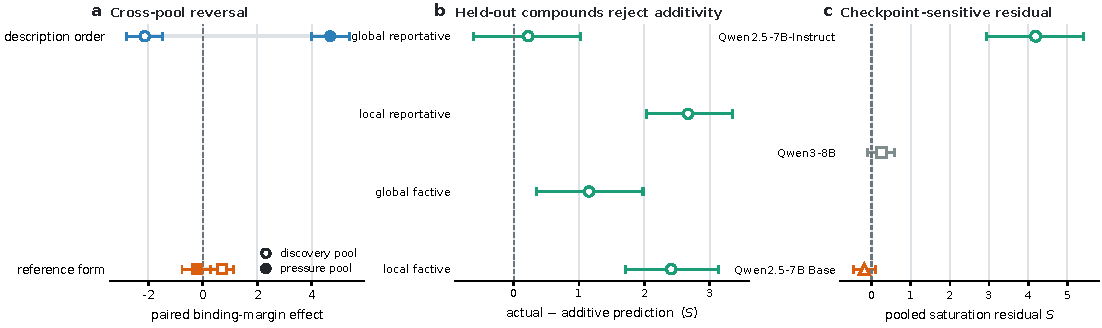
\includegraphics[width=\textwidth]{figures/figure_empirical_evidence.pdf}
    \caption{\textbf{Empirical closure of the source-accessibility argument.}
    (a) Discovery and item-disjoint pressure pools produce incompatible pooled
    wording effects. Open and filled markers denote the two pools; intervals are
    95\% item-cluster bootstrap intervals. (b) On four unseen passive-by-
    embedding compounds, actual responses exceed the frozen additive prediction
    in the positive residual direction. (c) The pooled saturation residual is
    directional only for Qwen2.5-7B-Instruct; Qwen3-8B and matched Qwen2.5-7B
    Base preserve a weaker control-relative preference but not the directional
    law.}
    \label{fig:empirical-evidence}
\end{figure*}

\section{Discussion}

% Plan: State the methodological implication and identify the paper's unit of analysis.
The central implication is methodological: answer accuracy is not an identifying
measurement of belief use. A model can preserve accuracy while changing which
described source controls the answer, or lose accuracy because a linguistic
construction restricts access to the correct source. Typed competitors turn
that ambiguity into an estimable interaction. For linguistically grounded
evaluation, the relevant unit is therefore not a paraphrase average but a
triple: the intended source, the competing source types, and the construction
that regulates access between description and answer.

% Plan: Interpret the held-out residual as a composition result while preserving the operator boundary.
The second implication is theoretical. Linguistic restrictions need not compose
as independent penalties. In Qwen2.5-7B-Instruct, voice and embedding constraints
share a behavioral bottleneck: their joint cost is smaller than the sum of their
isolated costs. This is stronger than documenting another sensitivity because
the additive account predicts unseen compounds and fails quantitatively. At the
same time, positive residuals identify only a subadditive class. The data do not
distinguish a weakest-link rule from every smooth saturating alternative, and
they do not imply that the model represents accessibility as a scalar variable.

% Plan: Explain the checkpoint result as a boundary on transfer rather than a causal training claim.
The checkpoint comparison adds a third implication. The typed source-control
object remains useful outside the positive checkpoint, but its composition law
is not portable in direction or magnitude. Because affine readout scaling would
preserve residual sign and normalized geometry, the failed transfer indicates a
functional change in how linguistic constraints reach the answer interface.
The matched Base contrast makes instruction tuning a plausible source of that
change, but only an association rather than a causal training result.

% Plan: State limitations as claim boundaries, not as a defensive experiment log.
These boundaries define the paper's scope. The stimuli are controlled synthetic
English worlds, the answer interface uses audited single-token candidates, and
the dependent variable is model behavior rather than human interpretation. We
therefore do not claim unrestricted English generality, broad model-family
transfer, human source-monitoring equivalence, or a hidden-state belief circuit.
The linguistic validity audit further treats grammaticality, source identity,
commitment, and target invariance as properties to be independently checked,
not assumed from generator intent.

% Plan: Close with the single transferable research question and the next scientific test.
\section{Conclusion}

This paper reframes linguistic sensitivity in theory-of-mind evaluation as a
source-binding problem. Typed conflict probes make the answer controller
identifiable, a frozen compound test reveals subadditive composition, and the
checkpoint comparison shows that this law is a boundary-sensitive behavioral
property rather than a portable model-family invariant. The next test is not
another paraphrase grid, but a controlled transfer of the typed geometry across
models or languages while freezing the same primitive costs. The central
question is therefore which linguistic systems make a source govern an answer,
and how those systems compose.


\bibliographystyle{plainnat}
\bibliography{references}

\appendix
\section{Evidence Inventory and Main Estimates}
\label{app:evidence-inventory}

The main text is organized by the hypotheses that survive falsification rather
than by execution order. For completeness, Table~\ref{tab:experiment-inventory}
lists every evidence matrix and its scientific role. The principal estimates
are shown in Table~\ref{tab:key-estimates} in the main text; this appendix
focuses on the complete cell-level audit and reproducibility details.

\begin{table}[H]
\centering
\small
\setlength{\tabcolsep}{4pt}
\renewcommand{\arraystretch}{1.08}
\begin{tabularx}{\textwidth}{@{}Xrr>{\raggedright\arraybackslash}X@{}}
\toprule
Evidence matrix & Worlds/groups & Score rows & Scientific role \\
\midrule
Surface-axis discovery & 80 & 880 & Discovery: pooled wording effects \\
Independent pressure pool & 80 & 880 & Falsification: pooled portability \\
Same-world topology cross & 30 & 1,980 & Confirmation: typed conflict moderation \\
Four-realization cross & 30 & 7,920 & Confirmation: realization boundary \\
Construction factorial & 30 & 2,160 & Localization: voice, locality, source type \\
Unseen compound forms & 30 & 1,440 & Prediction: frozen additive costs \\
New latent worlds & 20 & 1,440 & Independent saturation confirmation \\
\midrule
Total & -- & 16,700 & Distinct interventions across evidence chain \\
\bottomrule
\end{tabularx}
\caption{Experimental inventory. Row count is reported to expose coverage, not as a substitute for independence: the final matrix uses new latent worlds and a preregistered inequality.}
\label{tab:experiment-inventory}
\end{table}


\section{Latent Worlds and Invariance Audits}
\label{app:latent-worlds}

% Plan: Specify the latent event schema that remains invariant across linguistic forms.
Each world contains a queried agent, a comparison agent, an optional role
decoy, a target object, an optional object decoy, source and destination
locations, an initial observation, a movement event, information available to
each agent, and a return/query event. The queried agent receives no information
about the critical move. Role conflict changes another agent's state; object
conflict introduces a competing object movement; joint conflict combines both.
The question and typed candidate set are generated from the latent record rather
than recovered from surface text.

% Plan: Explain block-level invariance and independence checks.
For every latent-world block, the generator verifies invariant candidate JSON,
target source, event manifest, object identity, queried agent, and exact context
length across all topologies and surface forms. The same-world topology source
contains 30 blocks and 180 source rows with zero invariant failures. The
four-realization source expands these to 720 exact-length rows before linguistic
arms. The final 20-world source has zero normalized latent-signature overlap
with the earlier 30-world pool. An earlier nominal replication with 80/80
identity-field overlap is explicitly classified as replay-equivalent and is not
used as held-out evidence.

\section{Linguistic Intervention Inventory}
\label{app:linguistic-arms}

% Plan: Present every controlled language arm and its intended operation.
\begin{table}[H]
\centering
\footnotesize
\begin{tabularx}{\textwidth}{llX}
\toprule
Axis & Arm & Controlled linguistic operation \\
\midrule
Description order & role-first & Identify the comparison character before excluding competing states. \\
Description order & state-first & Exclude reality and the queried belief before naming the comparison state. \\
Reference & name-explicit & Name both queried and comparison characters explicitly. \\
Reference & pronoun-resolved & Introduce the comparison character, then use a resolved pronoun. \\
Reference & pronoun-ambiguous & Present two characters and use an underspecified pronoun. \\
Negation/evidence & affirmative-direct & Affirmatively request the comparison character's belief. \\
Negation/evidence & negated-exclusion & Exclude queried belief and reality before requesting the target. \\
Negation/evidence & source-explicit & Frame the answer as following the comparison character's evidence. \\
Role label/name & role-label & Refer to comparison and queried agents only by role. \\
Role label/name & name-explicit & Replace role labels with character names. \\
\bottomrule
\end{tabularx}
\caption{Linguistic intervention inventory. The full prompt strings are generated deterministically from the latent world and are included in the released manifests.}
\label{tab:linguistic-arms}
\end{table}


% Plan: Give representative prompt contrasts so readers can inspect semantic preservation.
For description order, the role-first arm begins by identifying the comparison
character and then excludes the queried character and reality; the state-first
arm first excludes those competing states and only then names the comparison
belief. For reference form, the name-explicit arm names both characters, the
resolved-pronoun arm introduces the comparison character before using
``their,'' and the ambiguous arm introduces both characters before the same
pronoun. For evidential wording, the affirmative arm directly licenses the
comparison belief, the negated arm excludes queried belief and reality, and the
source-explicit arm distinguishes testimony, queried evidence, and actual
location. The full deterministic strings are retained in the stimulus
manifests, making lexical differences auditable.

\section{Complete Pooled and Cross-Pool Results}

% Plan: Expose all positive and negative pooled-effect replication outcomes.
\begin{table}[H]
\centering
\footnotesize
\setlength{\tabcolsep}{4pt}
\begin{tabularx}{\textwidth}{Xlrrrcc}
\toprule
Axis & Role & Discovery & Independent & Independent CI & Sign & Pass \\
\midrule
Description order & Primary & -2.132 & 4.678 & [3.990, 5.374] & 0 & 0 \\
Reference form & Primary & 0.705 & -0.227 & [-0.762, 0.306] & 0 & 0 \\
Negation/evidence & Control & 0.541 & 4.143 & [3.326, 4.948] & 1 & 0 \\
Role label/name & Control & -0.328 & -1.238 & [-1.761, -0.676] & 1 & 0 \\
\bottomrule
\end{tabularx}
\caption{Independent-pool audit of pooled language effects. No primary axis passes the frozen portability gate; this failure motivates conditioning on typed conflict topology.}
\label{tab:cross-pool}
\end{table}


% Plan: Clarify why the failed controls matter to the story.
The independent pressure pool reverses the description-order effect and removes
the reference-form effect. Negation/evidential wording and role-label versus
name also violate their designated null/ratio gates. We therefore do not select
or refit a ``stable'' wording axis on this pool. Its role is falsification of a
pressure-invariant main-effect account.

\section{Complete Same-World Topology Results}

% Plan: Report all axes, both context lengths, and exploratory status.
\begin{table}[H]
\centering
\footnotesize
\setlength{\tabcolsep}{4pt}
\begin{tabularx}{\textwidth}{Xrrrrcc}
\toprule
Axis & Interaction & Bootstrap interval & 1,024 & 2,048 & Stable & Pass \\
\midrule
Description order & 6.722 & [5.697, 7.747] & 6.338 & 7.105 & 1 & 1 \\
Reference form & -1.062 & [-1.724, -0.409] & -1.042 & -1.083 & 1 & 1 \\
Negation/evidence & 3.706 & [2.875, 4.527] & 4.763 & 2.648 & 1 & 1 \\
Role label/name & -1.966 & [-2.600, -1.317] & -1.726 & -2.206 & 1 & 0 \\
\bottomrule
\end{tabularx}
\caption{Same-world typed-conflict interactions. The three preregistered axes pass with direction stability at both context lengths; role-label versus name remains exploratory. Intervals are 95\% percentile item-cluster bootstrap intervals.}
\label{tab:same-item}
\end{table}


% Plan: Explain how context-length stability is assessed.
Length stability requires the sign of the joint-minus-single interaction to
agree at 1,024 and 2,048 tokens. All four axes meet this descriptive condition,
but only the three preregistered axes are eligible for confirmatory promotion.
The role-label effect is therefore visible rather than discarded, while its
post-hoc status remains explicit.

\section{Complete Cross-Realization Results}

% Plan: Report the full three-axis by four-template matrix.
\begin{table}[H]
\centering
\footnotesize
\setlength{\tabcolsep}{4pt}
\begin{tabularx}{\textwidth}{Xrrrrr}
\toprule
Axis & Canonical & Event log & Reportative & Indirect & Aggregate / bootstrap interval \\
\midrule
Description order & 6.308 & 0.813 & 5.876 & 5.205 & 4.551 [3.907, 5.152] \\
Reference form & -0.780 & -1.946 & -0.142 & -1.156 & -1.006 [-1.474, -0.530] \\
Negation/evidence & 3.963 & 2.200 & -1.052 & 0.473 & 1.396 [0.915, 1.896] \\
\bottomrule
\end{tabularx}
\caption{Topology interactions across four realization families. The reportative negation reversal is the construction boundary that motivates the accessibility factorial. Aggregate intervals are 95\% percentile item-cluster bootstrap intervals.}
\label{tab:multitemplate}
\end{table}


% Plan: Distinguish sign stability from directional-confidence stability.
Description order retains the predicted sign in all four realizations but the
structured event-log interval includes zero. Reference form likewise keeps its
sign throughout, with an interval crossing zero for the event-wise report.
Negation/evidential wording reverses under event-wise reportative embedding and
is weak under compact indirect report. The aggregate gate passes because its
interval is directional and at least three realization means retain the
predicted sign; the mixed cells remain central to the accessibility argument.

\section{Construction Factorial}

% Plan: Report every primitive cell and factorial contrast used to derive costs.
\begin{table}[H]
\centering
\footnotesize
\setlength{\tabcolsep}{4pt}
\begin{tabularx}{\textwidth}{lXrrr}
\toprule
Estimand & Contrast/form & $n$ & Mean & Bootstrap interval \\
\midrule
Form effect & Active, unembedded & 30 & 3.606 & [2.670, 4.574] \\
Form effect & Passive, unembedded & 30 & 0.653 & [-0.342, 1.596] \\
Form effect & Global reportative & 30 & 2.588 & [1.840, 3.369] \\
Form effect & Local reportative & 30 & -0.473 & [-1.246, 0.267] \\
Form effect & Global factive & 30 & 1.918 & [1.138, 2.727] \\
Form effect & Local factive & 30 & -0.113 & [-0.730, 0.508] \\
Factorial contrast & Passive $-$ active & 30 & -2.952 & [-4.037, -1.796] \\
Factorial contrast & Reportative locality & 30 & -3.061 & [-4.267, -1.911] \\
Factorial contrast & Factive locality & 30 & -2.032 & [-3.221, -0.908] \\
Factorial contrast & Reportative-specific locality & 30 & -1.030 & [-1.945, -0.097] \\
\bottomrule
\end{tabularx}
\caption{Complete construction-factorial results. Negative contrasts denote reduced topology-moderated control relative to the named baseline. Intervals are 95\% percentile item-cluster bootstrap intervals over latent worlds.}
\label{tab:factorial}
\end{table}


% Plan: State the exact interpretation boundary of the factorial.
The factorial identifies separable behavioral losses associated with agent
demotion, local embedding, and reportative-specific locality. It does not show
that local reportative embedding alone yields a reliably negative topology
effect, and it does not identify a hidden-state scope or source-monitoring
module. Its scientific role is to define primitive construction costs and a
held-out composition problem.

\section{Frozen Compound Prediction}

% Plan: Show all unseen compound forms and their residuals.

% Plan: Document how the frozen prediction avoids fitting each held-out item.
For each held-out item and construction, the additive prediction combines the
item's active-construction effect with a leave-one-item-out mean voice cost from
the factorial pool. Thus the target item does not contribute to its own voice
cost. The no-voice control uses the corresponding active construction without
the estimated voice penalty. Additive sign prediction is broadly correct, but
its aggregate error does not improve over that control.

\section{Saturation-Model Comparison}

% Plan: Expose the complete post-hoc model comparison and operator non-identifiability.
\begin{table}[H]
\centering
\footnotesize
\setlength{\tabcolsep}{4pt}
\begin{tabularx}{\textwidth}{XrrcX}
\toprule
Predictor & MAE / gain & Gain interval & Directional pass & Interpretation \\
\midrule
No Voice predictor & 2.153 & -- & -- & absolute error \\
Additive predictor & 2.260 & -- & -- & absolute error \\
Average predictor & 1.599 & -- & -- & absolute error \\
Weakest Link predictor & 1.453 & -- & -- & absolute error \\
Wrong Max predictor & 2.616 & -- & -- & absolute error \\
\midrule
weakest link vs additive & 0.807 & [0.363, 1.247] & 1 & distinguished \\
weakest link vs no voice & 0.700 & [0.406, 1.028] & 1 & distinguished \\
weakest link vs average & 0.146 & [-0.204, 0.440] & 0 & not distinguished \\
weakest link vs wrong max & 1.162 & [0.780, 1.543] & 1 & distinguished \\
\bottomrule
\end{tabularx}
\caption{Post-hoc predictor comparison on the first held-out compounds. Saturating predictors beat additivity, but weakest-link does not beat average saturation; the unique operator is therefore not identified. Gain intervals are 95\% percentile item-cluster bootstrap intervals.}
\label{tab:model-comparison}
\end{table}


% Plan: Define each comparison model in prose.
The additive predictor sums primitive costs. The no-voice predictor ignores the
voice cost. Average saturation predicts the mean of the two primitive
construction effects. Weakest-link uses the smaller topology effect, equivalent
to the larger primitive cost under the present sign convention. Wrong-max uses
the opposite extreme as a specificity control. Weakest-link and average
saturation both improve over additivity, while their direct comparison is
unresolved; no unique min, max, or tropical law is claimed.

\section{Independent Saturation Confirmation}

% Plan: Report every confirmatory estimand and control gain on new worlds.
\begin{table}[H]
\centering
\footnotesize
\setlength{\tabcolsep}{3pt}
\begin{tabular}{lrrrrrr}
\toprule
Predicate & Saturation & Interval & Weakest gain & Interval & Average gain & Interval \\
\midrule
reportative & 4.609 & [2.646, 6.447] & 3.078 & [2.029, 4.203] & 3.606 & [2.366, 4.895] \\
factive & 3.771 & [2.274, 5.228] & 2.142 & [0.988, 3.362] & 2.689 & [1.373, 4.009] \\
\bottomrule
\end{tabular}
\caption{Independent confirmation on 20 new latent worlds. Positive saturation and predictive gains replicate for both predicate families. Intervals are 95\% percentile item-cluster bootstrap intervals over latent worlds.}
\label{tab:independent-saturation}
\end{table}


% Plan: Restate the preregistered gate and its outcome.
The confirmatory gate requires positive lower bounds for the saturation
residual, weakest-link gain, and average-saturation gain in both predicate
families. All six lower bounds are positive. The confirmation establishes
subadditivity while intentionally leaving the competition between saturation
operators unresolved.

\section{Cross-Checkpoint Affine-Gain Null}

The frozen 1,440-row confirmation manifest was scored without prompt, fit, or
gate changes on Qwen3-8B. Its pooled directional residual is not distinguishable
from zero, while both pooled control-relative predictor gains remain positive
(Table~\ref{tab:main-checkpoint-boundary}). The directional law therefore does not
replicate, motivating a narrower question: is the difference merely a scalar
readout-gain change?

\input{../../results/oral_readiness_pack_20260707/affine_gain_null_audit_20260805/affine_gain_invariance_theorem}

We fit the affine map using only active, passive, and local primitive forms in
four training folds and predict the held-out compound and residual in the
fifth. Aligned predictions are compared with target-mean, item-shuffled,
zero-residual, and wrong-predicate controls. The gate fails for both predicate
families (Table~\ref{tab:affine-gain}). Thus Qwen3 exhibits amplitude
compression and partial control-relative shape transfer, but not an
affine-rescaled copy of the Qwen2.5-Instruct saturation geometry.

\begin{table}[H]
\centering
\small
\begin{tabular}{lrrrrc}
\toprule
Predicate & Slope & Compound MAE & Gain vs. mean & Residual $r$ & Gate \\
\midrule
Reportative & 0.068 & 0.483 & $-0.055$ [$-0.146$, 0.032] & 0.203 & fail \\
Factive & 0.061 & 0.491 & $-0.130$ [$-0.252$, $-0.020$] & 0.124 & fail \\
\bottomrule
\end{tabular}
\caption{Five-fold primitive-only affine transport from Qwen2.5-7B-Instruct
to Qwen3-8B. Positive gain would mean the aligned predictor improves over a
training-fold target-mean control. Neither predicate passes the full affine
gain gate.}
\label{tab:affine-gain}
\end{table}



\section{Statistical Procedure}
\label{app:statistics}

% Plan: Detail within-item reduction and cluster resampling.
The primitive observation is a latent world, not an individual prompt row. For
each axis and construction, paired arm differences are computed within the same
parent stimulus. Topology interactions are then computed within world and
context length; the two lengths are averaged to form one value per world.
Bootstrap resampling draws worlds with replacement and carries every associated
arm, topology, construction, and length together. Reported intervals are the
2.5th and 97.5th percentiles of 8,000 bootstrap means.

% Plan: Explain directional gates and model-comparison gains.
Directional gates compare the full confidence interval with zero in the
preregistered direction. Predictor gains are paired absolute-error differences,
so a positive gain means the named predictor has lower error than its comparator
on the same world and compound form. No row-level independent-sample test is
used. The final pooled saturation interval resamples the predicate-specific
world residuals with the same fixed analysis seed used in the released audit.

\section{Model Scoring and Reproducibility}
\label{app:reproducibility}

% Plan: Give exact model-loading and scoring details needed to reproduce logits.
The primary matrices use Qwen2.5-7B-Instruct revision
\newline\texttt{a09a35458c702b33eeacc393d103063234e8bc28}. Frozen transfer uses
Qwen3-8B revision
\newline\texttt{b968826d9c46dd6066d109eabc6255188de91218} and Qwen2.5-7B Base
revision \newline\texttt{d149729398750b98c0af14eb82c78cfe92750796}. Scoring uses Hugging Face
Transformers in offline mode, float16 weights, automatic device mapping,
12~GiB GPU and 48~GiB CPU memory limits, batch size one for the final
construction matrices, and CPU offload when required. The scorer requests only
the final-position logits, computes log-softmax once, and indexes the audited
single-token candidates. Checkpointed CSV writing and resume-by-stimulus ID do
not change completed rows.

% Plan: Document deterministic generation and audit surfaces.
Latent-world generation, neutral padding, linguistic-arm rendering, template
rendering, bootstrap resampling, and source-overlap checks use fixed seeds.
Every manifest stores the full prompt, target block, candidate JSON, target
source, context target and realized lengths, tokenizer-based candidate counts,
latent signature, template/construction labels, and parent stimulus ID. Each
analysis emits both a complete matrix and a machine-readable decision file.
The manuscript tables are generated directly from these matrices rather than
transcribed manually.

\section{Claim Boundary and Theorem-to-Experiment Map}

% Plan: State the exact safe and unsafe claim surfaces before mapping them to evidence.
The paper supports a controlled, behavioral source-accessibility saturation law
within Qwen2.5-7B-Instruct and a checkpoint-sensitive composition boundary
across the tested Qwen checkpoints.
It does not claim a hidden-state source-monitoring circuit, a portable causal
belief controller, human psycholinguistic universality, broad model-family
transfer, unrestricted English generality, or a unique aggregation operator.

% Plan: Separate formal identities, empirical inequalities, and blocked mechanisms.
\begin{table}[H]
\centering
\small
\begin{tabular}{p{0.25\linewidth}p{0.25\linewidth}p{0.38\linewidth}}
\toprule
Statement & Status & Evidence and boundary \\
\midrule
Topology-moderated effect & Defined and measured & Same-item role, object, and joint conflict crosses; no universality claim. \\
Cost-residual identity & Proved & Exact under Definitions~\ref{def:topology-effect}--\ref{def:saturation-residual}. \\
Saturating-composition bound & Conditional proof & Holds for nonnegative costs and an aggregator between maximum and sum; does not assert a neural implementation. \\
Reportative residual $>0$ & Independently validated & 20 new latent items; the interval remains entirely above zero. \\
Factive residual $>0$ & Independently validated & 20 new latent items; the interval remains entirely above zero. \\
Unique min/tropical operator & Not identified & Weakest-link does not reliably beat average saturation. \\
Affine readout-gain transfer & Rejected & Primitive-only five-fold transport fails both predicate gates on Qwen3-8B. \\
Matched Base directional law & Not replicated & The pooled interval crosses zero; both pooled predictor-control gates remain positive. \\
\bottomrule
\end{tabular}
\vspace{4pt}
\caption{Separation of algebraic statements, empirical inequalities, and blocked mechanism claims.}
\label{tab:theorem-evidence}
\end{table}


% Required NeurIPS paper checklist; it follows the references and appendix.
\newpage
\section*{NeurIPS Paper Checklist}

%%% BEGIN INSTRUCTIONS %%%

{\bf The checklist answers are an integral part of your paper submission.} They are visible to the reviewers, area chairs, senior area chairs, and ethics reviewers. You will also be asked to include it (after eventual revisions) with the final version of your paper, and its final version will be published with the paper.

The reviewers of your paper will be asked to use the checklist as one of the factors in their evaluation. While \answerYes{} is generally preferable to \answerNo{}, it is perfectly acceptable to answer \answerNo{} provided a proper justification is given (e.g., error bars are not reported because it would be too computationally expensive'' or ``we were unable to find the license for the dataset we used''). In general, answering \answerNo{} or \answerNA{} is not grounds for rejection. While the questions are phrased in a binary way, we acknowledge that the true answer is often more nuanced, so please just use your best judgment and write a justification to elaborate. All supporting evidence can appear either in the main paper or the supplemental material, provided in appendix. If you answer \answerYes{} to a question, in the justification please point to the section(s) where related material for the question can be found.

IMPORTANT, please:
\begin{itemize}
    \item {\bf Delete this instruction block, but keep the section heading ``NeurIPS Paper Checklist"},
    \item  {\bf Keep the checklist subsection headings, questions/answers and guidelines below.}
    \item {\bf Do not modify the questions and only use the provided macros for your answers}.
\end{itemize} 
 

%%% END INSTRUCTIONS %%%


\begin{enumerate}

\item {\bf Claims}
    \item[] Question: Do the main claims made in the abstract and introduction accurately reflect the paper's contributions and scope?
    \item[] Answer: \answerYes{}
    \item[] Justification: The abstract and introduction state the typed source-control contribution, the checkpoint-sensitive saturation result, and the explicit non-claims about hidden circuits and instruction-tuning causality.
    \item[] Guidelines:
    \begin{itemize}
        \item The answer \answerNA{} means that the abstract and introduction do not include the claims made in the paper.
        \item The abstract and/or introduction should clearly state the claims made, including the contributions made in the paper and important assumptions and limitations. A \answerNo{} or \answerNA{} answer to this question will not be perceived well by the reviewers. 
        \item The claims made should match theoretical and experimental results, and reflect how much the results can be expected to generalize to other settings. 
        \item It is fine to include aspirational goals as motivation as long as it is clear that these goals are not attained by the paper. 
    \end{itemize}

\item {\bf Limitations}
    \item[] Question: Does the paper discuss the limitations of the work performed by the authors?
    \item[] Answer: \answerYes{}
    \item[] Justification: The Discussion and Conclusion state the synthetic-English, single-token, checkpoint, model-family, and hidden-state-mechanism boundaries.
    \item[] Guidelines:
    \begin{itemize}
        \item The answer \answerNA{} means that the paper has no limitation while the answer \answerNo{} means that the paper has limitations, but those are not discussed in the paper. 
        \item The authors are encouraged to create a separate ``Limitations'' section in their paper.
        \item The paper should point out any strong assumptions and how robust the results are to violations of these assumptions (e.g., independence assumptions, noiseless settings, model well-specification, asymptotic approximations only holding locally). The authors should reflect on how these assumptions might be violated in practice and what the implications would be.
        \item The authors should reflect on the scope of the claims made, e.g., if the approach was only tested on a few datasets or with a few runs. In general, empirical results often depend on implicit assumptions, which should be articulated.
        \item The authors should reflect on the factors that influence the performance of the approach. For example, a facial recognition algorithm may perform poorly when image resolution is low or images are taken in low lighting. Or a speech-to-text system might not be used reliably to provide closed captions for online lectures because it fails to handle technical jargon.
        \item The authors should discuss the computational efficiency of the proposed algorithms and how they scale with dataset size.
        \item If applicable, the authors should discuss possible limitations of their approach to address problems of privacy and fairness.
        \item While the authors might fear that complete honesty about limitations might be used by reviewers as grounds for rejection, a worse outcome might be that reviewers discover limitations that aren't acknowledged in the paper. The authors should use their best judgment and recognize that individual actions in favor of transparency play an important role in developing norms that preserve the integrity of the community. Reviewers will be specifically instructed to not penalize honesty concerning limitations.
    \end{itemize}

\item {\bf Theory assumptions and proofs}
    \item[] Question: For each theoretical result, does the paper provide the full set of assumptions and a complete (and correct) proof?
    \item[] Answer: \answerYes{}
    \item[] Justification: Methodology states the definitions and assumptions; the cost-residual identity and saturating-composition bound are proved in the main text and mapped to Appendix~L.
    \item[] Guidelines:
    \begin{itemize}
        \item The answer \answerNA{} means that the paper does not include theoretical results. 
        \item All the theorems, formulas, and proofs in the paper should be numbered and cross-referenced.
        \item All assumptions should be clearly stated or referenced in the statement of any theorems.
        \item The proofs can either appear in the main paper or the supplemental material, but if they appear in the supplemental material, the authors are encouraged to provide a short proof sketch to provide intuition. 
        \item Inversely, any informal proof provided in the core of the paper should be complemented by formal proofs provided in appendix or supplemental material.
        \item Theorems and Lemmas that the proof relies upon should be properly referenced. 
    \end{itemize}

    \item {\bf Experimental result reproducibility}
    \item[] Question: Does the paper fully disclose all the information needed to reproduce the main experimental results of the paper to the extent that it affects the main claims and/or conclusions of the paper (regardless of whether the code and data are provided or not)?
    \item[] Answer: \answerYes{}
    \item[] Justification: Methodology fixes the model, tokenizer, candidate interface, context lengths, estimands, bootstrap unit, and confirmatory gates; Appendix~K gives scoring and reproducibility details.
    \item[] Guidelines:
    \begin{itemize}
        \item The answer \answerNA{} means that the paper does not include experiments.
        \item If the paper includes experiments, a \answerNo{} answer to this question will not be perceived well by the reviewers: Making the paper reproducible is important, regardless of whether the code and data are provided or not.
        \item If the contribution is a dataset and\slash or model, the authors should describe the steps taken to make their results reproducible or verifiable. 
        \item Depending on the contribution, reproducibility can be accomplished in various ways. For example, if the contribution is a novel architecture, describing the architecture fully might suffice, or if the contribution is a specific model and empirical evaluation, it may be necessary to either make it possible for others to replicate the model with the same dataset, or provide access to the model. In general. releasing code and data is often one good way to accomplish this, but reproducibility can also be provided via detailed instructions for how to replicate the results, access to a hosted model (e.g., in the case of a large language model), releasing of a model checkpoint, or other means that are appropriate to the research performed.
        \item While NeurIPS does not require releasing code, the conference does require all submissions to provide some reasonable avenue for reproducibility, which may depend on the nature of the contribution. For example
        \begin{enumerate}
            \item If the contribution is primarily a new algorithm, the paper should make it clear how to reproduce that algorithm.
            \item If the contribution is primarily a new model architecture, the paper should describe the architecture clearly and fully.
            \item If the contribution is a new model (e.g., a large language model), then there should either be a way to access this model for reproducing the results or a way to reproduce the model (e.g., with an open-source dataset or instructions for how to construct the dataset).
            \item We recognize that reproducibility may be tricky in some cases, in which case authors are welcome to describe the particular way they provide for reproducibility. In the case of closed-source models, it may be that access to the model is limited in some way (e.g., to registered users), but it should be possible for other researchers to have some path to reproducing or verifying the results.
        \end{enumerate}
    \end{itemize}


\item {\bf Open access to data and code}
    \item[] Question: Does the paper provide open access to the data and code, with sufficient instructions to faithfully reproduce the main experimental results, as described in supplemental material?
    \item[] Answer: \answerNo{}
    \item[] Justification: The current anonymous submission does not yet provide a public code or data URL; the appendix documents the manifests, generators, and exact scoring protocol for an anonymized release.
    \item[] Guidelines:
    \begin{itemize}
        \item The answer \answerNA{} means that paper does not include experiments requiring code.
        \item Please see the NeurIPS code and data submission guidelines (\url{https://neurips.cc/public/guides/CodeSubmissionPolicy}) for more details.
        \item While we encourage the release of code and data, we understand that this might not be possible, so \answerNo{} is an acceptable answer. Papers cannot be rejected simply for not including code, unless this is central to the contribution (e.g., for a new open-source benchmark).
        \item The instructions should contain the exact command and environment needed to run to reproduce the results. See the NeurIPS code and data submission guidelines (\url{https://neurips.cc/public/guides/CodeSubmissionPolicy}) for more details.
        \item The authors should provide instructions on data access and preparation, including how to access the raw data, preprocessed data, intermediate data, and generated data, etc.
        \item The authors should provide scripts to reproduce all experimental results for the new proposed method and baselines. If only a subset of experiments are reproducible, they should state which ones are omitted from the script and why.
        \item At submission time, to preserve anonymity, the authors should release anonymized versions (if applicable).
        \item Providing as much information as possible in supplemental material (appended to the paper) is recommended, but including URLs to data and code is permitted.
    \end{itemize}


\item {\bf Experimental setting/details}
    \item[] Question: Does the paper specify all the training and test details (e.g., data splits, hyperparameters, how they were chosen, type of optimizer) necessary to understand the results?
    \item[] Answer: \answerYes{}
    \item[] Justification: The paper specifies the fixed checkpoint, prompt construction, typed candidate sets, context lengths, held-out split, scoring rule, and frozen prediction protocol in Methodology and Appendix~K.
    \item[] Guidelines:
    \begin{itemize}
        \item The answer \answerNA{} means that the paper does not include experiments.
        \item The experimental setting should be presented in the core of the paper to a level of detail that is necessary to appreciate the results and make sense of them.
        \item The full details can be provided either with the code, in appendix, or as supplemental material.
    \end{itemize}

\item {\bf Experiment statistical significance}
    \item[] Question: Does the paper report error bars suitably and correctly defined or other appropriate information about the statistical significance of the experiments?
    \item[] Answer: \answerYes{}
    \item[] Justification: Main tables and figures report item-cluster bootstrap intervals; Methodology defines the latent-world sampling unit and fixed resampling procedure.
    \item[] Guidelines:
    \begin{itemize}
        \item The answer \answerNA{} means that the paper does not include experiments.
        \item The authors should answer \answerYes{} if the results are accompanied by error bars, confidence intervals, or statistical significance tests, at least for the experiments that support the main claims of the paper.
        \item The factors of variability that the error bars are capturing should be clearly stated (for example, train/test split, initialization, random drawing of some parameter, or overall run with given experimental conditions).
        \item The method for calculating the error bars should be explained (closed form formula, call to a library function, bootstrap, etc.)
        \item The assumptions made should be given (e.g., Normally distributed errors).
        \item It should be clear whether the error bar is the standard deviation or the standard error of the mean.
        \item It is OK to report 1-sigma error bars, but one should state it. The authors should preferably report a 2-sigma error bar than state that they have a 96\% CI, if the hypothesis of Normality of errors is not verified.
        \item For asymmetric distributions, the authors should be careful not to show in tables or figures symmetric error bars that would yield results that are out of range (e.g., negative error rates).
        \item If error bars are reported in tables or plots, the authors should explain in the text how they were calculated and reference the corresponding figures or tables in the text.
    \end{itemize}

\item {\bf Experiments compute resources}
    \item[] Question: For each experiment, does the paper provide sufficient information on the computer resources (type of compute workers, memory, time of execution) needed to reproduce the experiments?
    \item[] Answer: \answerNo{}
    \item[] Justification: The paper specifies model and inference configuration but does not yet report a complete per-experiment hardware and wall-clock ledger; this will be included with the reproducibility artifact.
    \item[] Guidelines:
    \begin{itemize}
        \item The answer \answerNA{} means that the paper does not include experiments.
        \item The paper should indicate the type of compute workers CPU or GPU, internal cluster, or cloud provider, including relevant memory and storage.
        \item The paper should provide the amount of compute required for each of the individual experimental runs as well as estimate the total compute. 
        \item The paper should disclose whether the full research project required more compute than the experiments reported in the paper (e.g., preliminary or failed experiments that didn't make it into the paper). 
    \end{itemize}
    
\item {\bf Code of ethics}
    \item[] Question: Does the research conducted in the paper conform, in every respect, with the NeurIPS Code of Ethics \url{https://neurips.cc/public/EthicsGuidelines}?
    \item[] Answer: \answerYes{}
    \item[] Justification: The study uses synthetic latent worlds and pretrained-model inference, involves no human subjects or sensitive personal data, and reports negative and boundary results without overstating causal mechanisms.
    \item[] Guidelines:
    \begin{itemize}
        \item The answer \answerNA{} means that the authors have not reviewed the NeurIPS Code of Ethics.
        \item If the authors answer \answerNo, they should explain the special circumstances that require a deviation from the Code of Ethics.
        \item The authors should make sure to preserve anonymity (e.g., if there is a special consideration due to laws or regulations in their jurisdiction).
    \end{itemize}


\item {\bf Broader impacts}
    \item[] Question: Does the paper discuss both potential positive societal impacts and negative societal impacts of the work performed?
    \item[] Answer: \answerYes{}
    \item[] Justification: The Discussion identifies the benefit of more diagnostic linguistic evaluation and the risk of over-interpreting behavioral source control as human-like belief reasoning or a hidden causal circuit.
    \item[] Guidelines:
    \begin{itemize}
        \item The answer \answerNA{} means that there is no societal impact of the work performed.
        \item If the authors answer \answerNA{} or \answerNo, they should explain why their work has no societal impact or why the paper does not address societal impact.
        \item Examples of negative societal impacts include potential malicious or unintended uses (e.g., disinformation, generating fake profiles, surveillance), fairness considerations (e.g., deployment of technologies that could make decisions that unfairly impact specific groups), privacy considerations, and security considerations.
        \item The conference expects that many papers will be foundational research and not tied to particular applications, let alone deployments. However, if there is a direct path to any negative applications, the authors should point it out. For example, it is legitimate to point out that an improvement in the quality of generative models could be used to generate Deepfakes for disinformation. On the other hand, it is not needed to point out that a generic algorithm for optimizing neural networks could enable people to train models that generate Deepfakes faster.
        \item The authors should consider possible harms that could arise when the technology is being used as intended and functioning correctly, harms that could arise when the technology is being used as intended but gives incorrect results, and harms following from (intentional or unintentional) misuse of the technology.
        \item If there are negative societal impacts, the authors could also discuss possible mitigation strategies (e.g., gated release of models, providing defenses in addition to attacks, mechanisms for monitoring misuse, mechanisms to monitor how a system learns from feedback over time, improving the efficiency and accessibility of ML).
    \end{itemize}
    
\item {\bf Safeguards}
    \item[] Question: Does the paper describe safeguards that have been put in place for responsible release of data or models that have a high risk for misuse (e.g., pre-trained language models, image generators, or scraped datasets)?
    \item[] Answer: \answerNA{}
    \item[] Justification: The paper does not release a new pretrained model, scraped dataset, or high-risk deployment artifact.
    \item[] Guidelines:
    \begin{itemize}
        \item The answer \answerNA{} means that the paper poses no such risks.
        \item Released models that have a high risk for misuse or dual-use should be released with necessary safeguards to allow for controlled use of the model, for example by requiring that users adhere to usage guidelines or restrictions to access the model or implementing safety filters. 
        \item Datasets that have been scraped from the Internet could pose safety risks. The authors should describe how they avoided releasing unsafe images.
        \item We recognize that providing effective safeguards is challenging, and many papers do not require this, but we encourage authors to take this into account and make a best faith effort.
    \end{itemize}

\item {\bf Licenses for existing assets}
    \item[] Question: Are the creators or original owners of assets (e.g., code, data, models), used in the paper, properly credited and are the license and terms of use explicitly mentioned and properly respected?
    \item[] Answer: \answerNo{}
    \item[] Justification: The Qwen checkpoint and cited prior assets are credited, but the current manuscript does not yet include a complete asset-by-asset license ledger; this remains a submission-artifact gap.
    \item[] Guidelines:
    \begin{itemize}
        \item The answer \answerNA{} means that the paper does not use existing assets.
        \item The authors should cite the original paper that produced the code package or dataset.
        \item The authors should state which version of the asset is used and, if possible, include a URL.
        \item The name of the license (e.g., CC-BY 4.0) should be included for each asset.
        \item For scraped data from a particular source (e.g., website), the copyright and terms of service of that source should be provided.
        \item If assets are released, the license, copyright information, and terms of use in the package should be provided. For popular datasets, \url{paperswithcode.com/datasets} has curated licenses for some datasets. Their licensing guide can help determine the license of a dataset.
        \item For existing datasets that are re-packaged, both the original license and the license of the derived asset (if it has changed) should be provided.
        \item If this information is not available online, the authors are encouraged to reach out to the asset's creators.
    \end{itemize}

\item {\bf New assets}
    \item[] Question: Are new assets introduced in the paper well documented and is the documentation provided alongside the assets?
    \item[] Answer: \answerYes{}
    \item[] Justification: The synthetic latent-world schema, linguistic intervention axes, manifests, gates, and evidence inventory are documented in Methods and Appendices B--L.
    \item[] Guidelines:
    \begin{itemize}
        \item The answer \answerNA{} means that the paper does not release new assets.
        \item Researchers should communicate the details of the dataset\slash code\slash model as part of their submissions via structured templates. This includes details about training, license, limitations, etc. 
        \item The paper should discuss whether and how consent was obtained from people whose asset is used.
        \item At submission time, remember to anonymize your assets (if applicable). You can either create an anonymized URL or include an anonymized zip file.
    \end{itemize}

\item {\bf Crowdsourcing and research with human subjects}
    \item[] Question: For crowdsourcing experiments and research with human subjects, does the paper include the full text of instructions given to participants and screenshots, if applicable, as well as details about compensation (if any)? 
    \item[] Answer: \answerNA{}
    \item[] Justification: The study contains no crowdsourcing or human-subject experiment.
    \item[] Guidelines:
    \begin{itemize}
        \item The answer \answerNA{} means that the paper does not involve crowdsourcing nor research with human subjects.
        \item Including this information in the supplemental material is fine, but if the main contribution of the paper involves human subjects, then as much detail as possible should be included in the main paper. 
        \item According to the NeurIPS Code of Ethics, workers involved in data collection, curation, or other labor should be paid at least the minimum wage in the country of the data collector. 
    \end{itemize}

\item {\bf Institutional review board (IRB) approvals or equivalent for research with human subjects}
    \item[] Question: Does the paper describe potential risks incurred by study participants, whether such risks were disclosed to the subjects, and whether Institutional Review Board (IRB) approvals (or an equivalent approval/review based on the requirements of your country or institution) were obtained?
    \item[] Answer: \answerNA{}
    \item[] Justification: The study contains no human participants and therefore required no IRB review.
    \item[] Guidelines:
    \begin{itemize}
        \item The answer \answerNA{} means that the paper does not involve crowdsourcing nor research with human subjects.
        \item Depending on the country in which research is conducted, IRB approval (or equivalent) may be required for any human subjects research. If you obtained IRB approval, you should clearly state this in the paper. 
        \item We recognize that the procedures for this may vary significantly between institutions and locations, and we expect authors to adhere to the NeurIPS Code of Ethics and the guidelines for their institution. 
        \item For initial submissions, do not include any information that would break anonymity (if applicable), such as the institution conducting the review.
    \end{itemize}

\item {\bf Declaration of LLM usage}
    \item[] Question: Does the paper describe the usage of LLMs if it is an important, original, or non-standard component of the core methods in this research? Note that if the LLM is used only for writing, editing, or formatting purposes and does \emph{not} impact the core methodology, scientific rigor, or originality of the research, declaration is not required.
    %this research? 
    \item[] Answer: \answerYes{}
    \item[] Justification: A pretrained language model is the evaluated object; its checkpoint, tokenizer, inference interface, and role in the experiments are described in Methodology.
    \item[] Guidelines:
    \begin{itemize}
        \item The answer \answerNA{} means that the core method development in this research does not involve LLMs as any important, original, or non-standard components.
        \item Please refer to our LLM policy in the NeurIPS handbook for what should or should not be described.
    \end{itemize}

\end{enumerate}


\end{document}
